\subsection{Functional failure study}
\label{sec:failure-case-study}

%TODO: Speak about impact (or no) of positive stress. Say that only neg stress causes a restart

% What is the failure
The failure is observed on the V\textsubscript{2p5} output pin (Fig. \ref{fig:meas-reset-v2p5}).
It affects the behavior of the entire system, because this net powers many other functions in the system.
The failure is induced by injecting a large negative-voltage stress on the input V\textsubscript{batt}, when the product is in operation.
The discharge is superimposed on a DC voltage value.
This input is a realistic entry point for \gls{esd} in the integrated circuit, because it is exposed at the system level and connected to the battery by a cable.
The disturbance on the output V\textsubscript{2p5} is much longer (30 \textmu{}s) than on the input V\textsubscript{batt} (100 ns).
It seems the negative stress is triggering a reset of the regulator.

%TODO: MEASUREMENT of the output during failure
\begin{figure}[!htbp]
  \centering
  \includegraphics{src/3/figures/measure_v2p5.png}
  \caption{Measurement of V\textsubscript{2p5} after a negative stress}
  \label{fig:meas-reset-v2p5}
\end{figure}

% What is the root cause -> reset of regulator, soft-start
It seems that the negative stress is causing an unwanted \gls{soft-start} sequence in the regulator.
A soft-start normally happens only during system power-up, when the main external supply is switched on.
During a soft-start, the supply voltage slowly rises from 0V to its nominal value.
It avoids overshoots that could damage sensitive blocks.
By design, soft-starts require a large amount of time to complete, in the range of tens to hundreds microseconds.
As a consequence, the function is not available, or at least not considered valid, until the soft-start is finished.

% How is the test conducted
To generate the negative stress, a \gls{tlp} generator is employed.
The simulations use the \gls{tlp} model described previously in section \ref{sec:tlp-modeling}).
The injection is performed with DPI pattern (ref?).
Basically, the stress and DC supply are isolated from one another with a capacitor-inductor network.
The injection setup is given in Fig. \ref{fig:sim-setup-reset}.

%TODO: Injection setup with injection pattern
\begin{figure}[!htbp]
  \centering
  \includegraphics{src/3/figures/injection_setup_simulations.png}
  \caption{Simulation setup to reproduce the reset}
  \label{fig:sim-setup-reset}
\end{figure}

% Are the simulations accurate
%TODO: Detail more
In a first step, it is checked if the reset is reproduced correctly by simulation.
V\textsubscript{batt} and V\textsubscript{2p5} simulations are compared with measurements in Fig. \ref{fig:wvf-vbatt} and Fig. \ref{fig:wvf-v2p5}.
Both curves correlate well, and the regulator restart is correctly reproduced in simulation.
These results tend to indicate that the simulations can be trusted for this study case.

% TODO: MEASUREMENT vs SIMULATION
\begin{figure}[!htbp]
  \centering
  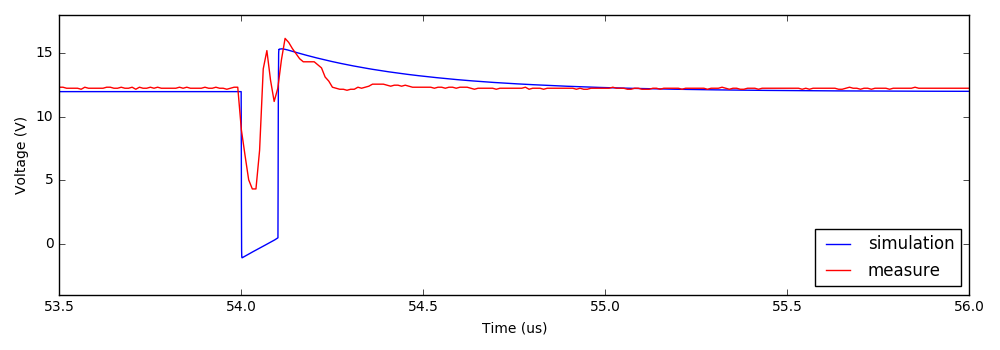
\includegraphics[width=0.9\textwidth]{src/3/figures/vbatt.png}
  \caption{Simulation versus measurement for V\textsubscript{batt}}
  \label{fig:wvf-vbatt}
\end{figure}

\begin{figure}[!htbp]
  \centering
  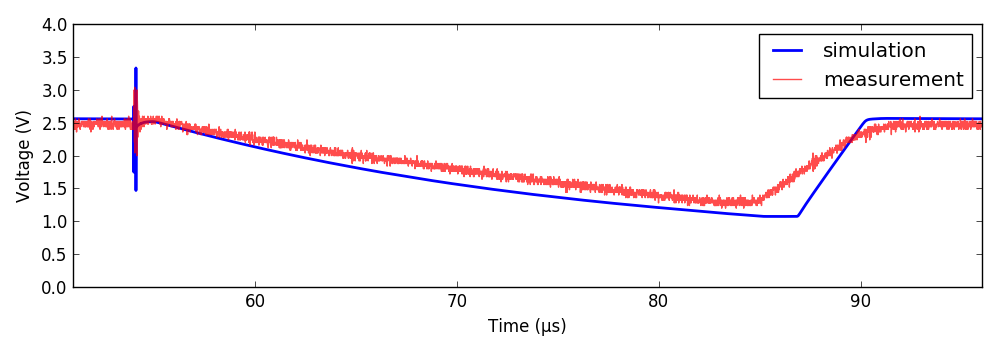
\includegraphics[width=0.9\textwidth]{src/3/figures/v2p5.png}
  \caption{Simulation versus measurement for V\textsubscript{2p5}}
  \label{fig:wvf-v2p5}
\end{figure}

% Now use the simulation for analysis
Since the simulation correctly reproduces the external input and output waveforms, it is used to observe the intermediate nets.
The simulation is run with a rectangular pulse of -100V amplitude and 100 ns width.
The waveform for output V\textsubscript{clamp9} of the pre-regulator is given in Fig. \ref{fig:wvf-vclamp9}.
At 54 \textmugreek{}s,  V\textsubscript{clamp9} is disturbed by the negative stress, in two phases.
The first phase is 100 ns wide, and corresponds to the direct exposure to the stress.
During this phase, V\textsubscript{clamp9} reaches as low as 0V for a brief amount of time.
Afterwards, there is a second phase, that lasts approximately 650 ns.
The reason for this second undervoltage is not clearly known, but it looks similar to the positive overshoot on the  V\textsubscript{batt} curve (Fig. \ref{fig:wvf-vbatt}).
Overall, V\textsubscript{clamp9} is disturbed for 750 ns.

\begin{figure}[!htbp]
  \centering
  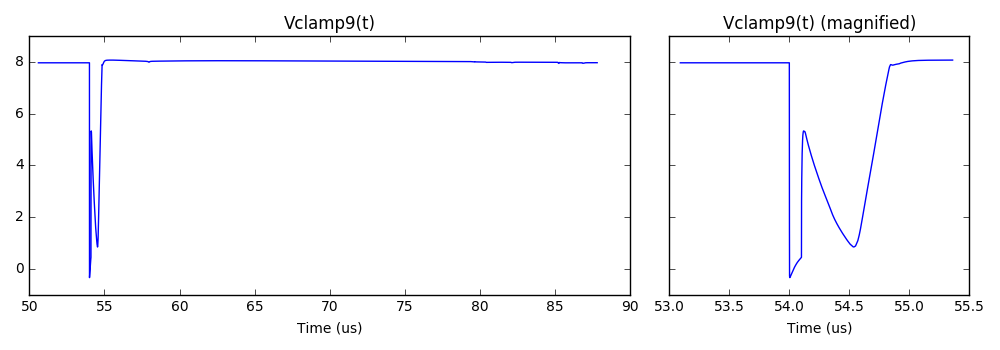
\includegraphics[width=0.9\textwidth]{src/3/figures/vclamp9.png}
  \caption{Simulated waveform of the V\textsubscript{clamp9} internal net}
  \label{fig:wvf-vclamp9}
\end{figure}

% Next net, bandgap input
V\textsubscript{clamp9} is used as input for powering the bandgap reference.
In turn, the bandgap is expected to be disturbed as well.
The observation of the 1.0V bandgap reference V\textsubscript{ref1p0} confirms it (Fig. \ref{fig:wvf-v1p0}).
The reference drops down to 0.25V, and is disturbed for about 3 \textmugreek{}s.

\begin{figure}[!htbp]
  \centering
  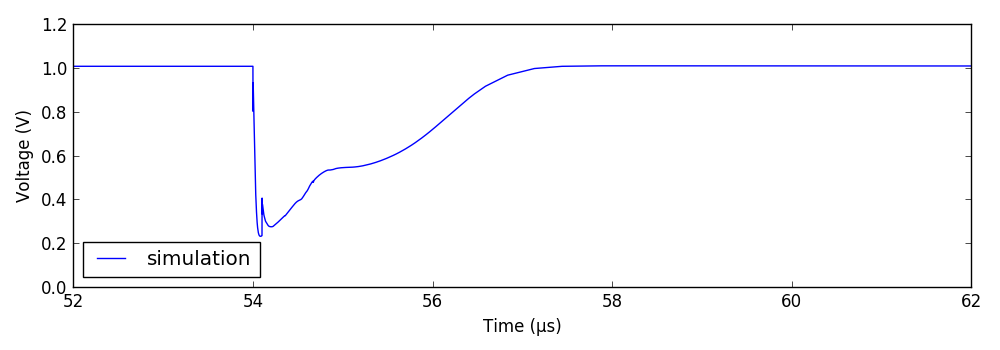
\includegraphics[width=0.9\textwidth]{src/3/figures/v1p0.png}
  \caption{Simulated waveform of the V\textsubscript{ref1p0} internal net}
  \label{fig:wvf-v1p0}
\end{figure}

% Final net
Finally, V\textsubscript{ref1p0} is used by the regulator to generate the 2.5 V external supply output V\textsubscript{2p5}.
Previously,  Fig. \ref{fig:wvf-v2p5} showed that V\textsubscript{2p5} drops below 1.5V, and is disturbed for more than 30 \textmugreek{}s.

% Preliminary conclusion with scale factor
There is a clear trend regarding the duration of the failure.
In the first block (pre-regulator), the disturbance width increased from 100 ns to 750 ns.
In the second block (bandgap), it increased from 750 ns to 3 \textmugreek{}s.
In the third block (regulator), it reached 30 \textmugreek{}s.
Each time, there is an aggravation of the failure.

% Talk about failure in cascade
To conclude, it appears there is a failure in cascade of the regulation function.
When the disturbance propagates through a block, it is amplified and becomes more severe.
Ultimately, a function that takes a lot of time to recover (soft-start) is hit, causing a full system restart.

The next part of this research work is focused on acquiring measurement data on silicon, to confirm the simulations.
Also, this study case remains simple to understand, but fixing the issue is difficult.
It must be ensured that a circuit correction for \gls{esd} does not affect normal operation.
In practice this can be difficult, because both can have opposite requirements.
There are also many situations where the failure cause is not so obvious, and calls for advanced investigation methods.

For these purposes a testchip is designed in next section \ref{sec:test-vehicle-desc}.
Modeling methods are explored in section \ref{sec:bottom-up-modeling} as a way to understand better these issues.
